\subsection{Компилятор} \label{sub111}

Компилятор~--- это программа, которая  принимает текст программы, написанной на одном языке~--- \textit{исходном}, и транслирует (переводит) его в эквивалентный текст на другом языке~--- \textit{целовом}. Одна из важных ролей компилятора состоит в сообщении об ошибках в исходной программе, обнаруженных в процессе трансляции.

Процесс компиляции можно разделить на две большие части. Первая часть~--- \textit{анализ} разбивает исходную программу на составные части и накладывает на них грамматическую структуру. Затем он использует эту структуру для промежуточного представления программы. Анализ сообщает пользователю об ошибках, собирает информацию об исходной программе и сохраняет её в \textit{таблице символов}. Вторая часть~--- \textit{синтез}, строит требуемую целевую программу на основе промежуточного представления и информации из таблицы символов.

Фаза анализа компиляции разделена на лексический и синтаксический анализ по ряду причин: 

\begin{enumerate} 
	\item{Упрощение разработки. Отделение лексического анализа от синтаксического позволяет упростить как минимум одну из фаз анализа. Например, включить в синтаксический анализатор работу с комментариями и пробельными символами существенно сложнее, чем удалить их лексическим анализатором.}
	\item{Увеличение эффективности компилятора. Отдельный лексический анализатор позволяет применять более специализированные методики, предназначенные исключительно для решения лексических задач.}
	\item{Увеличение переносимости компилятора. Особенности устройств ввода могут быть ограниченны лексическим анализатором.}
\end{enumerate}

Если рассмотреть процесс компиляции более детально, можно увидеть, что он представляет собой последовательность фаз, каждая из которых преобразует одно представление программы в другое:

\begin{itemize}
\item{\textit{Лексический анализ} или \textit{сканирование}. Лексический анализатор читает поток символов, составляющих исходную программу, группирует их в значащие последовательности (лексемы), формирует для каждой лексемы специальные структуры данных, называемые токенами и передает их синтаксическому анализатору.}	
\item{\textit{Синтаксический анализ} или \textit{разбор}. Синтаксический анализатор использует использует информацию из предыдущей фазы и на её основе строит синтаксическое дерево, в котором каждый внутренний узел представляет операцию, а дочерние узлы~--- аргументы этой операции.}	
\item{\textit{Семантический анализ}. Эта фаза компиляции аспользует синтаксическое дерево и информацию из таблицы символов для проверки исходной программы на семантическую согласованность с определением языка. Важной частью семантического анализа является проверка и приведение типов.}	
\item{\textit{Генерация промежуточного кода.} На этой фазе компилятор генерирует низкоуровневое промежуторчное представление кода исходной программы, которое можно рассматривать как программу для абстрактной вычислительной машины.}	
\item{\textit{Оптимизация кода.} Фаза машинно-независимой оптимизации кода пытается улучшить промежуточный код.}	
\item{\textit{Генерация кода.} В качестве исходных данных генератор кода получает промежуточное представление исходной программы и отображает его в целевой язык, как правило в ассемблерный код.}		
\end{itemize}

%\begin{figure}[ht]
%	\centering
%	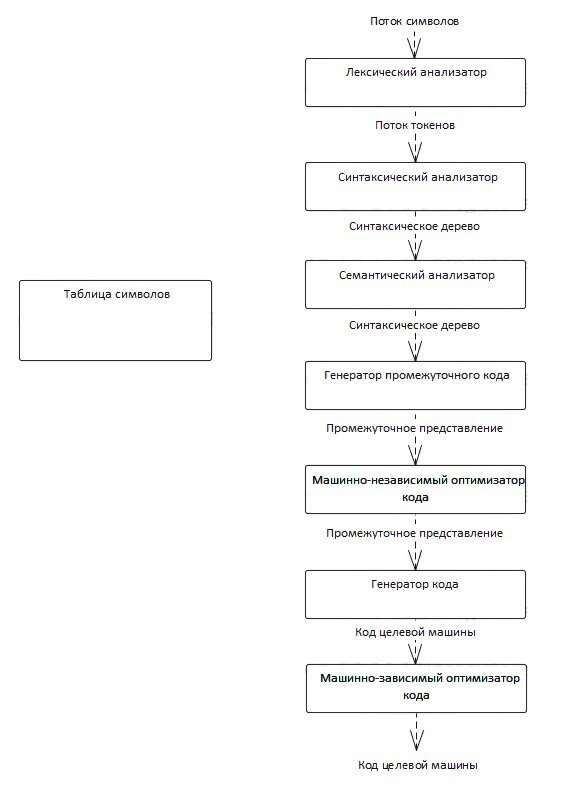
\includegraphics [scale=0.5] {compiler}
%	\caption{Схема взаимодействия фаз компилятора.}
%	\label{img:compiler}
%\end{figure}